\documentclass[12pt,letterpaper]{article}

\usepackage{amsmath, amsthm}
\usepackage{microtype, parskip}
\usepackage[comma,numbers,sort&compress]{natbib}
\usepackage{lineno}
\usepackage{docmute}
\usepackage{caption, subcaption, multirow, morefloats, rotating}
\usepackage{wrapfig}
\usepackage{attrib}

\frenchspacing

\begin{document}

\section*{Introduction}

\begin{quotation}
  All the world's a stage, And all the men and women merely players; They have their exits and their entrances\dots
\end{quotation}
\attrib{Shakespeare, \textit{As You Like It}, Act II, Scene VII}

% regional species pool

A regional species pool is the set of species which form communities in a specific region; local communities are subsets of the regional pool. The composition of a regional species pool changes over time due to speciation, migration, extinction. Local scale processes like resource competition only affect the regional species pool if all communities are affected.

How do species pools change over time as species are recruited or go extinct? When are specific species ecologies enriched or depleted in the environment? How does global and regional environmental context affect the distribution of species ecotypes (e.g. guilds) in a regional species pool? All of these questions fall under a single umbrella of analysis of ecotypic diversity and diversification.

% guilds and ecocube and ecotypes
Guilds are a set of species with similar sets of interactions and interactors (i.e. macroecology) \citep{Valentine1969,Bambach1977}. Species within a guild are expected to have more similar macroecological dynamics than species in different builds. Building on the framework of guilds, \citep{Bush2007} presented an ecocube for describing the position, motility, and trophic role of marine invertebrates. Unique combinations along the three ecological trait axes represent which among the possible ecotypes are observed. This approach has proven quite popular as it attempts to operationalize the guild in terms of shared characteristics \citep{Bush2007,Bambach2007,Bush2011}, but the overall utility of this approach is limited due to its condition as just a data type.

% how we think about mammal diversity
Analysis of mammal diversity and hypotheses as to the processes that have shaped it tend to fall into one or more of the following categories: diversity of an entire system (e.g. continent) \citep{Alroy2000g,Alroy1996a,Figueirido2012,Liow2008}, guild based \citep{Janis2004,Janis2000,Jernvall2004,Janis1993c,Pires2015a,Janis2008a}, clade based \citep{Quental2013,Slater2015c,Silvestro2015b}, climate based \citep{Blois2009,Janis1993c,Janis1993b}, and location based \citep{Eronen2015,Badgley2013}. Rarely are more than two of these categories considered simultaneously, and instead integration of these diverse observations and hypotheses tends to be based on coincidence. One of the goals of this study is to present a framework for simultaneously analyzing a diversity of hypotheses by pulling  information from multiple levels of organization by integrating both species traits and environmental factors into a single analysis in order to infer a more holistic picture of the processes which may have shaped mammal species diversity.

% what we're dealing with in terms of hypotheses
In the analyses done here, a few key covariates which describe species' macroecology and environmental context are considered. Because of the complexity inherent in this question and related analysis in terms of both number of covariates considered and structure of each model, it is possible to consider and test a large number of possible hypotheses. The analytical approach used here is appropriate for mitigating complications arising from this complexity (e.g. multiple comparisons, garden of forking paths) CITATIONS.

The principle species trait considered in this study is a species' ecotype, defined here as the unique combination of species dietary cateogry and locomotor category (e.g. arboreal omnivore versus unguligrade herbivore). This classification can be considered analogous to a guild or unique ecocube combination as discussed above \citep{Bush2007,Bambach2007,Bush2011}. Species mass was also included as a species trait, but is mostly included in order to control for that effect on species observation and occurrence.

There is no previous evidence of any major turnover events in history of North American mammal diversity, unlike the Neogene record European mammals \citep{Alroy2009,Alroy1996a,Eronen2015,Janis1993b,Alroy2000g}. There is also little evidence for simultaneous changes in cross-ecotype or cross-guild diveristy. Instead, turnover is distributed through time. It is then expected then that turnover events or periods of rapid diversification or depletion should not occur simultaneously for all ecotypes.

% hypotheses about the effect of ecotypes
%   difficult to tease out because people use taxonomic grouping, which conflates common ancestry and ecology
% things people have remarked upon in the past
%   cursorial carnivores are a late occurrence (Janis and Wilhelm 93 JME)
%   ungulate legs get longer over Cenozoic but due to climate change (Janis 08)
%   guilds stable in face of turnover EUROPE (jernvall and fortelius 04 amnat)
%   larger body size, greater extinction rate (liow et al 08 pnas)
%   ungulate extinction/turnover at end of eocene (janis 97)
%   browse to graze within herbivores
Translating previous work into hypotheses applicable to this analysis is difficult for a variety of reasons. Taxonomic groupings such as order or family are frequently invoked as an important factor in many proposed hypotheses for how mammal diversity is structured \citep{Quental2013,Slater2015c,Janis1993c,Pires2015a,Janis2008a}. Because taxonomic grouping conflates both species macroecology or guild membership with shared evolutionary history, there are no clear hypotheses as to macroecological change viewed through the lens of species interactions. Specifically, this issue arrises when trying to generalize previous observations from taxony-based to ecology-based hypotheses.

\citet{Jernvall2004} found that for the Neogene of Europe the relative abundance of mammal guilds was stable over time even in the face of high turnover rates, though they only considered large bodied taxa from a small set or mammal orders. Similar results have been observed for some taxonomic groups in North America CITATIONS.

Many discussions of the effects or associates of species ecology and diversity have focused on ungulate herbivores \citep{Janis2004,Janis2000,Janis1993c,Janis2008a} and carnivores \citep{Pires2015a,Slater2015c,Janis1993c,Silvestro2015b}.

The diversity history of ungulate herbivores is characterized by more recently originating taxa having longer legs, higher crowned teeth, and a shift from graze-dominated to browse-dominated diets than their earlier originating counterparts \citep{Janis2004,Janis2000,Janis1993c,Janis2008a}; all of which have all been attributed to some combination of environmental change and tectonic activity driving that environmental change \citep{Janis2008a,Eronen2015,Blois2009}. Additionally, it has been observed that ungulate cursorial forms arose prior to cursorial carnivore forms, an observation attributed to the reorganization of plant communities towards the end of the Cenozoic and the latter emergence of ``modern'' environments and communities \citep{Janis1993c}.

Within the canid guild of North America (e.g. plantigrade and digitigrade carnivores) there is evidence that their diversity is self-regulating or somehow limited. Specifically, it has been proposed that different clades of ``canids'' have replaced each other as dominating that macroecological role in the species pool \citep{Silvestro2015b}. A pattern of generally constant diversity through time is also observed within the canid carnivore subguilds of hypercarnivore, hypocarnivore, and mesocarnivores even in the face of constant species turnover is consistent with limited possibility of increased diversity, even though there was no evidence of diversity-dependence in trait (e.g. body size) evolution \citep{Slater2015c}.

There is some uncertainty as to the effect of species body size on mammal diversity and aspects of the diversification processes, specifically extinction \citep{Liow2008,Liow2009,Tomiya2013,Smits2015b}. Species body size is frequently framed as an important biological descriptor because of how correlated this trait is with other traits such as metabolic rate and home range size CITATIONS.It is also relatively easy to estimate the body mass of extinct species using proxy measures and regression equations, as was done in this study (see below). However, body size is normally considered in other studies without reference to other ecological descriptors of the species CITATION, but see \citep{Smits2015b}. Additionally, this high amount of correlation between life history traits and body size limits processed-based inference and hypothesis testing because the actual mechanisms underlying any observed pattern are obscured.

\citet{Smits2015b} found several systematic differences in mammal species durations associated with various species traits. Omnivorous taxa were found to have, on average, a greater duration than other dietary categories. Additionally, arboreal taxa were found to have a shorter duration than other locomotor categories. An unresolved question from \citet{Smits2015b} is whether the greater extinction risk faced by arboreal is constant over time or if there was a change in extinction risk at the Paleogene/Neogene boundary. Each of these possible explanations for the results of \citet{Smits2015b} have clear and testable predictions for this analysis. Specifically, 1) the extinction risk arboreal taxa increased in the Neogene compared to the Paleogene, driving the average extinction risk of arboreal mammals up and leading to the loss of arboreal taxa from the species pool, or 2) if arboreal taxa have just a generally higher extinction risk than other ecotypes but have maintained a constant diversity for the Cenozoic. 

% if we control for one ecotype axis, what is variation along other axis?
% digitigrade vs unguligrade herbivores
% plantigrade vs digitigrade carnivores
% modernization of ecologies?
%   this is normally talked about in terms of taxonomic groups
%   how does this translate into ecologies?




% effect of climate on diversification process
Fundamentally, all species respond differently to climate and environmental change \citep{Blois2009}. Macroecological patterns are the similarities across species and the emergent properties of how species react to a similar ``stimulus.''

The effect of climate on diversity and the diversification process has been the focus of considerable research with many analyses favoring diversification being more biologically-mediated than climate-mediated \citep{Alroy1996a,Alroy2000g,Figueirido2012,Clyde1998a}. Both temporal and geographic scale of analysis can make a big difference in the interpretation of results. For example when the mammal fossil record analyzed at small temporal and geographic scales a correlation between diversity and climate are observable \citep{Clyde1998a}. However, when the record is analyzed at the scale of the continent and most of the Cenozoic there is no correlation with diversity and climate \citep{Alroy2000g}. This results, however, does not go against the idea that there may be short periods of correlation and that the correlation between diveristy and climate or even reverse direction over time; instead this result means that there is no single direction of correlation between diversity and climate \citep{Figueirido2012}. 

In the case of a fluctuating correlation between diversity and climate it is hard to make the argument of an actual causal link between the two without modeling the underlying ecological differences between species; when this analysis is based on diversity or taxonomy alone no mechanisms are possible to infer. Taxonomy, like body size, stands in for many important species traits to the point that mechanistic or process based inference is impossible. While emergent patterns might correspond to taxonomic goruping, this itself is an emergent phenomenon. Instead, by framing hypotheses in terms of species traits and their environmental context, these emergent phenomenon are actually being studied as opposed to be assumed. 

The Cenozoic is generally characterized by a global cooling trend and the development of polar ice-caps during the Neogene, though there are a few notable exceptions to this broad characterization \citep{Zachos2001,Zachos2008,Cramer2011}. The Cenozoic of North America is additionally characterized by an environmental transition from the closed, partially forested environments of the Paleogene to the savannah and grasslands environments of the Neogene \citep{Blois2009,Janis1993b,Janis2000,Stromberg2005}.

A lot of the climate and environmental changes obserd for North America have been attributed to tectonic activity and uplift \citep{Blois2009,Eronen2015,Janis2008a,Badgley2013} CITATIONS. Additionally, tectonic activity and uplift is considered the causal mechanism secondarily behind both the diversification process and trait evolution \citep{Blois2009,Badgley2013} CITATIONS. Tectonic uplift changes weather patterns (e.g. rain shadow) and mobilizes grit into the environment. Increased grit in the environment combined with decreased rain fall is considered the primary reason behind the trend of increased hypsodonty, or high crowned teeth, among herbivore groups over the Cenozoic of both North America and Europe CITATIONS.

The Eocene-Oligocene transition is associated with high extinction amongst ungulate taxa \citep{Janis2008a}. This period is also the transition from the Paleogene to the Neogene and from herbivores being browsing dominated to grazing dominated CITATION. This transition is marked by WHAT? This transition is associated globally with the appearance of ice caps WHERE? Additionally, this transition is marked by GRASS? There is an observed stability in estimates of global temperature from the E/O transition till the end of the Miocene; this is called the Mid-Miocene climatic optimum \citep{Zachos2001,Zachos2008}. The Mid-Miocene climatic optimum is bookended by periods of temperature decline. We would then expect that, for the Miocene, turnover and other diversification events would most likely be biologically mediated because of the constancy of climate, and that for groups that are driven primarily by environmental factors, the Miocene would be a period of marked by an absence of major changes to diversity or the diversification process.

The environmental factors included in this study are estimates of global tempreature and the changing floral groups present in North America across the Cenozoic. These covariates were chosen because they provide high level characterizations of the environmental context of the entire North American regional species pool for most of the Cenozoic. Importantly, the effects of a species ecotype on diversity are themselves modeled as functions of environmental factors (Fig. \ref{fig:concept_fourth_corner}) allowing for inference as to how species ecology mediates environmental context. 

% 4th corner as similar but different lens
Fourth-corner modeling is an approach to explaining the patterns of either species abundance or presence/absence as a product of species traits, environmental factors, and the interaction between traits and environment \citep{Brown2014c,Warton2015a,Pollock2012,Jamil2013} CITATION. In modern ecological studies, what is being modeled is species occurrences at localities distributed across a region \citep{Pollock2012,Jamil2013}. In this study, what is being modeled is the pattern of species occurrence over time for most of the Cenozoic in North America (Fig. \ref{fig:concept_fourth_corner}). These two approaches, modern and palentologicial, are different views of the same three-dimensional pattern: species at localities over time. The temporal limitations of modern ecological studies and difficulties with uneven spatial occurrences of fossils in paleontological studies means that these approaches are complimentary but reveal different patterns of how species are distributed in time and space.

\begin{figure}[ht]
  \centering
  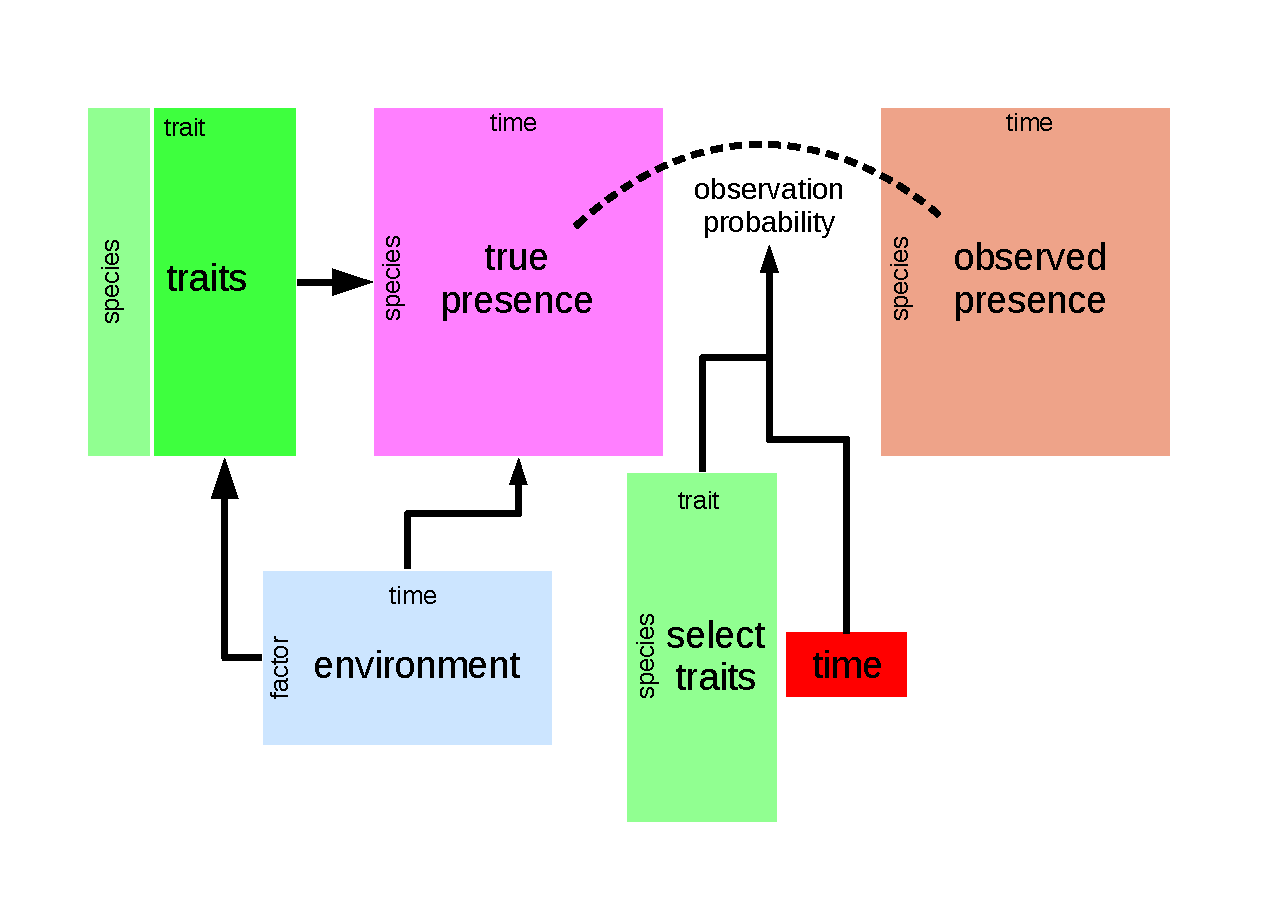
\includegraphics[width=\textwidth,height=0.8\textheight,keepaspectratio=true]{figure/paleo_fourth_corner}
  \caption[Conceptual diagram of the paleontological fourth-courner problem]{Conceptual diagram of the paleontological fourth corner problem. The observed presence matrix (orange) is the empirical presence/absence pattern for all species for all time points; this matrix is an incomplete observation of the ``true'' presence/absence pattern (purple). The estimated true presence matrix is modeled as a function of both environmental factors over time (blue) and multiple species traits (green). Additionally, the affect of environmental factors on species traits are also modeled as traits are expected to mediate the effects of a species environmental context. This diagram is based partially on material presented in \citet{Brown2014c} and \citet{Warton2015a}.}
  \label{fig:concept_fourth_corner}
\end{figure}

All observations, paleontological or modern, are made with uncertainty CITATIONS. With presernce/absence data this uncertainty comes from now knowing if an absence is a ``true'' absence or just a failure to observe \citep{Royle2008,Royle2014,Foote1999a,Foote2001,Lloyd2011,Wang2016b}. For paleontological data, the incomplete preservation of whatever species were present into fossil form combined with incomplete sampling of what fossils are present means that the true times of origination or extinction may not be observed \citep{Foote1999a,Foote2001,Wang2015,Wang2016b}.




% what have people said before
%   ungulates get hit at end of Eocene b/c cool (Janis 97)
%   climate is not correlated with mammal diversity or body size (Alroy et al 2000)
%   it is all mountain building (Badgley and Finarelli 13, Eronen et al 15 ProcB, Janis 93)
%     tectonic events drive climate, climate then affects species
%     taxonomic dependence






Ultimately, the goal of this analysis are to understand when are unique ecotypes enriched or depleted in the North American mammal regional species pool and how changes in ecotypic diversity are related to changes in species' environmental context.


\end{document}
